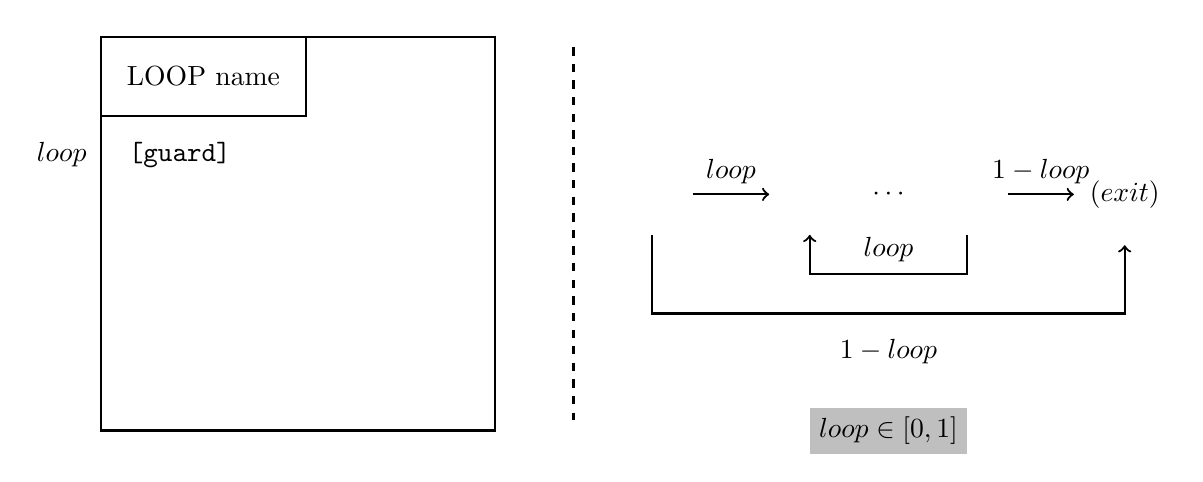
\begin{tikzpicture}[thick]
%%%%%%%%%%%%%%%%%%%%%%%%%%%%%%%%%%%%%%%%%%% HELP LINES
%\draw[help lines] (0,0) grid +(15,10);

%%%%%%%%%%%%%%%%%%%%%%%%%%%%%%%%%%%%%%%%%%% elements
\draw (1,0) rectangle +(5,5);
\node[shape=rectangle, draw=none](p1) at (0.5,3.5){$loop$};
\node[transparent] (t1) at (7,5){};
\node[transparent] (t2) at (7,0){};
\node[circle, dashed, minimum width=1cm] (current) at (8,3){};
\node[circle, minimum width=1cm] (s1) at (10,3){};
\node[circle, draw=none, minimum width=1cm] (s2) at (11,3){$\cdots$};
\node[circle, minimum width=1cm] (s3) at (12,3){};
\node[circle, minimum width=1cm] (s4) at (14,3){($exit$)};
\draw[dashed] (t1) -- (t2);
\draw[->,thick] (current) -- node[draw=none, above]{$loop$}(s1);
\draw[->,thick] (s3) -- node[draw=none, above]{$1-loop$}(s4);
\draw[->,thick] (s3.south) -- +(0,-0.5cm) -| (s1.south);
\node[rectangle, draw=none] at(11,2.3){$loop$};
\draw[->,thick] (current.south) -- +(0,-1cm) -| (s4.south);
\node[rectangle, draw=none] at(11,1){$1-loop$};

%%%%% guards and constraints
\node[shape=rectangle, draw=black, minimum height=1cm, minimum width=2.6cm](alt)at(2.3,4.5){LOOP name};
\node[shape=rectangle, draw=none](guard) at (2,3.5) {\texttt{[guard]}};
\node[shape=rectangle, fill=gray!50, draw=none](constraint) at (11,0) {$loop \in [0,1]$};


\end{tikzpicture}

